\documentclass[conference]{IEEEtran}
\IEEEoverridecommandlockouts
% ---------------------------------------------------------------
% Packages
% ---------------------------------------------------------------
\usepackage{cite}
\usepackage{amsmath,amssymb,amsfonts}
\usepackage{algorithmic}
\usepackage{graphicx}
\usepackage{textcomp}
\usepackage{xcolor}
\usepackage{booktabs}
\usepackage{multirow}
\usepackage{url}
\usepackage{balance}

\def\BibTeX{{\rm B\kern-.05em{\sc i}\kern-.025em b\kern-.08em
    T\kern-.1667em\lower.7ex\hbox{E}\kern-.125emX}}

\begin{document}

\title{Uncertainty-Aware Machine Learning Surrogates and SHAP-Guided Inverse Design for Melt-Crystal Interface Control in Vertical Bridgman Crystal Growth\\}

\author{
\IEEEauthorblockN{1\textsuperscript{st} Dr. R. AnandhaSree}
\IEEEauthorblockA{\textit{Dept. of Computer Science and Engineering} \\
\textit{Sathyabama Institute of Science and Technology}\\
Chennai, India \\
anandhasreer.cse@sathyabama.ac.in}
\and
\IEEEauthorblockN{2\textsuperscript{nd} Janardhanan Ramesh}
\IEEEauthorblockA{\textit{Dept. of Computer Science and Engineering} \\
\textit{Sathyabama Institute of Science and Technology}\\
Chennai, India \\
janardhananrameshh@gmail.com}
\and
\IEEEauthorblockN{3\textsuperscript{rd} Kalaipriya S}
\IEEEauthorblockA{\textit{Dept. of Computer Science and Engineering} \\
\textit{Sathyabama Institute of Science and Technology}\\
Chennai, India \\
kalaipriyaanjana99@gmail.com}
}

\maketitle

\begin{abstract}
Melt-crystal interface control is central to producing high-quality single crystals via the vertical Bridgman (VB) method, yet interface position and shape are difficult to observe or adjust in situ, and the physics-based numerical simulations used to study them are computationally expensive. This paper presents an uncertainty-aware, explainable machine learning framework for surrogate modeling and automated process design in a five-heater VB furnace growing BaBrCl crystal, directly extending the only prior machine-learning study built on this simulation dataset. Where that study compared two algorithms (linear regression and random forest) on two pooled output quantities, we independently model the centerline and edge interface positions ($L_c$, $L_e$) and their deflection ($D$) across seven regression algorithms under a leakage-free, five-fold cross-validation protocol, and select each target's model using a cross-validation-only, multi-metric ranking that never consults the held-out test set. A Gaussian Process Regression (GPR) surrogate dominates all three targets, achieving $R^2=0.994$ and $R^2=0.977$ for $L_c$ and $L_e$ respectively, while additionally providing calibrated predictive uncertainty that is absent from all prior work on this problem. For the substantially harder deflection target, we identify and resolve a methodological discrepancy with the reference study's reported performance by introducing a pooled cross-validation statistic directly comparable to theirs, closing most -- though not all -- of the apparent gap ($R^2$ improves from 0.665 under a mean-of-folds statistic to 0.713 under the pooled statistic, against a reported reference value of 0.78). We further validate our SHAP-based explainability results against the reference study's own SHAP findings, confirming independent agreement on the two dominant heaters governing interface deflection, while showing that engineered thermal-gradient features carry explanatory signal beyond any individual raw set-point. Finally, we replace the reference study's manual, non-systematic heater-adjustment procedure with an automated, uncertainty-penalized inverse-design optimizer based on differential evolution, which discovers heater set-points achieving a target interface deflection to within 0.2 mm without human intervention. All code, trained models, and results are made openly available for reproducibility.
\end{abstract}

\begin{IEEEkeywords}
machine learning, crystal growth, vertical Bridgman method, surrogate modeling, Gaussian process regression, explainable AI, SHAP, inverse design, uncertainty quantification, BaBrCl
\end{IEEEkeywords}

% =================================================================
\section{Introduction}
% =================================================================
The vertical Bridgman (VB) method remains one of the most widely used techniques for growing bulk single crystals from the melt \cite{bridgman}. As the ampoule is translated from the hot zone toward the cold zone, a melt-crystal interface separates the still-molten and already-solidified material. The macroscopic \emph{shape} and \emph{position} of this interface is a first-order determinant of the final crystal's quality: an interface that is moderately convex toward the melt minimizes thermoelastic stress and suppresses the nucleation of cracks and dislocations, while an interface that drifts or deforms during growth invites defect formation and non-uniform impurity distribution \cite{zhang_cheng2022}. Because the interface forms deep inside an opaque, high-temperature furnace, it cannot be observed directly during production, and adjusting it requires indirect control through the power delivered to a bank of independently controlled heaters.

Physics-based numerical simulation -- typically finite-volume or finite-element heat-transfer models such as CrysMAS -- has long been used to study how heater set-points shape the interface, and such models have been validated against experimental and neutron-imaging measurements for the BaBrCl system considered in this paper \cite{derby_neutron}. However, these simulations are slow, are typically operated in a forward direction only (set-points $\rightarrow$ interface shape), and offer no native mechanism for solving the \emph{inverse} problem of recommending set-points that achieve a desired interface outcome. This has motivated a growing body of work applying machine learning (ML) models, trained on simulation output, as fast surrogates for crystal-growth process design \cite{dropka_review}. Most such surrogates, however, are neural-network black boxes that offer no insight into \emph{why} a prediction was made, and few report calibrated predictive uncertainty -- a serious omission for any model intended to guide real process decisions.

The most directly relevant prior work is Zhang and Cheng \cite{zhang_cheng2022}, who trained linear regression (LR) and random forest (RF) models on a 96-point CrysMAS-simulated design of experiments for a five-heater VB furnace growing BaBrCl crystal, and used SHAP (SHapley Additive exPlanations) values to explain the RF model. Their study is a valuable proof of concept for explainable ML in crystal growth, but it has several limitations that we address directly in this paper: (i) it models only two \emph{pooled} output quantities -- average interface position $P$ and deflection $D$ -- rather than the physically distinct centerline and edge positions that determine them; (ii) it compares only two algorithms, neither of which reports predictive uncertainty; (iii) its own reported cross-validation statistic is ambiguous with respect to how out-of-fold predictions are aggregated, complicating exact reproduction; and (iv) its ``application to crystal growth practice'' is a manual exercise -- reading a SHAP plot by eye, proposing four candidate heater adjustments by hand, and checking them against scenarios already present in the training data -- rather than a systematic, automated search.

This paper makes the following contributions:
\begin{enumerate}
\item We independently model the centerline interface position $L_c$, edge interface position $L_e$, and interface deflection $D$ from the five heater set-points, comparing seven regression algorithms (linear regression, ridge regression, support vector regression, random forest, XGBoost, histogram-based gradient boosting, and Gaussian process regression) under an identical, leakage-free five-fold cross-validation protocol, with model selection performed strictly from cross-validation results and never from the held-out test set.
\item We introduce a \emph{pooled} cross-validation statistic, computed identically to what the reference study appears to report, alongside the conventional mean-of-folds statistic, enabling a direct, like-for-like comparison of our results to theirs and resolving a substantial fraction of an initially observed performance discrepancy.
\item We package the selected models as a fast, uncertainty-aware surrogate that reports calibrated predictive uncertainty via Gaussian process regression -- a capability absent from all prior machine-learning work on this system -- together with input/output range validation that flags extrapolation.
\item We compute SHAP explanations for our models and perform, to our knowledge, the first cross-study validation of SHAP-derived physical insight in this domain, confirming independent agreement with the reference study on the dominant heaters governing interface deflection while showing that engineered thermal-gradient features carry signal beyond the raw set-points used in prior work.
\item We replace the reference study's manual heater-adjustment procedure with an automated, uncertainty-penalized inverse-design optimizer that searches for heater set-points achieving a specified interface outcome, subject to the physical ordering constraint required for directional solidification.
\end{enumerate}

The remainder of this paper is organized as follows. Section~II reviews related work. Section~III describes the dataset and problem formulation. Section~IV details the complete methodology. Section~V presents and discusses results. Section~VI states limitations, and Section~VII concludes.

% =================================================================
\section{Related Work}
% =================================================================
Physics-based simulation of Bridgman and related melt-growth processes has a long history, from early one-dimensional analytical thermal models \cite{naumann1982} to modern finite-volume codes such as CrysMAS that resolve two-dimensional, axis-symmetric temperature fields under conductive and radiative heat transfer \cite{crysmas_manual}. Such simulations have been validated against physical measurements of BaBrCl and BaBrCl:Eu crystals grown in VB furnaces, including via energy-resolved neutron imaging \cite{derby_neutron}, giving confidence that simulation-trained models capture behavior representative of the real process.

Machine learning has increasingly been applied on top of such simulations to accelerate crystal-growth process design, including predicting interface shape and position \cite{dang2019}, growth rate \cite{takehara2021}, furnace temperature fields \cite{dropka2019}, and melt flow \cite{tsunooka2018}. The large majority of these studies employ artificial neural networks \cite{dropka_review}, which achieve strong predictive accuracy but function as black boxes, offering no direct insight into which process variables drive a given prediction -- a serious limitation when the goal is to \emph{guide}, not merely predict, manufacturing decisions.

Explainable machine learning addresses this gap by attaching interpretable structure to otherwise opaque models. SHAP, grounded in cooperative game theory, quantifies each input feature's contribution to each individual prediction and has been shown to recover globally consistent, locally faithful explanations for tree-ensemble models \cite{lundberg2017,lundberg2020}. Zhang and Cheng \cite{zhang_cheng2022} were, to our knowledge, among the first to apply SHAP specifically to a crystal-growth prediction problem, explaining a random forest model of interface position and deflection for the same BaBrCl VB system and dataset used in this paper. Our work is a direct methodological extension of theirs, detailed model-by-model in Section~IV and compared quantitatively in Section~V.

% =================================================================
\section{Dataset and Problem Formulation}
% =================================================================
\subsection{Furnace and Dataset}
The dataset used in this study was generated by CrysMAS simulation of a five-heater VB furnace growing BaBrCl crystal, an alkaline-halide scintillator material of interest for medical and security applications \cite{yan2016}. The furnace's five heaters -- top, upper, middle, lower, and bottom -- are independently controlled to set-point temperatures $T_1,\ldots,T_5$ respectively, each measured in kelvin at a thermocouple positioned at the heater's mid-height. For each combination of set-points, CrysMAS solves the steady-state heat-diffusion equation under radiative and conductive heat transfer to determine the temperature field, from which the melt-crystal interface -- the isotherm at BaBrCl's melting point, $T_{mp}=1168\,$K -- is extracted \cite{zhang_cheng2022}.

Two positions on this interface are recorded: $L_c$, its position at the ampoule centerline ($r=0$), and $L_e$, its position at the ampoule wall ($r=6.5\,$mm). From these, two derived quantities are also reported: the average position $P=(L_c+L_e)/2$ and the deflection $D=L_c-L_e$, where $D>0$ indicates a convex interface (favorable, lower thermal stress) and $D<0$ indicates a concave interface.

A full-factorial design over the levels shown for each heater in the source furnace design would yield $3^3\times 2^2=108$ combinations; the physical requirement that $T_1\geq T_2\geq T_3\geq T_4\geq T_5$ -- a positive axial temperature gradient, necessary to drive directional solidification downward -- eliminates 12 infeasible combinations, leaving $n=96$ simulated operating points, each with five inputs and four recorded quantities ($L_c$, $L_e$, $P$, $D$).

\subsection{Target Selection and Data Verification}
Before any modeling was performed, we verified programmatically that $P=(L_c+L_e)/2$ and $D=L_c-L_e$ hold exactly across all 96 rows (maximum absolute deviation on the order of $10^{-17}$, consistent with floating-point round-off). This confirms that $P$ carries no information beyond $L_c$ and $L_e$ and is therefore excluded from modeling as redundant, while $D$, although algebraically derivable from $L_c$ and $L_e$, is modeled \emph{directly} as an independent regression target -- consistent with the reference study's own treatment of deflection as a primary output of interest, and because a model trained directly on $D$ is not forced to inherit compounding error from two upstream predictions. This verification step is reported here explicitly because rigorous confirmation of a dataset's documented column semantics against the data itself, prior to any modeling, is a basic but frequently skipped element of reproducible ML research.

We therefore model $L_c$, $L_e$, and $D$ as three regression targets, each a function of the five heater set-points $T_1,\ldots,T_5$.

% =================================================================
\section{Methodology}
% =================================================================
\subsection{Preprocessing and Leakage Prevention}
The dataset contains no missing values and no duplicate rows; every row corresponds to a distinct combination of heater set-points. An interquartile-range (IQR) screen identifies one to three rows per target as statistical outliers, but inspection shows these correspond to the most extreme corner points of the temperature design, not measurement or simulation error, and they are retained rather than removed. All modeling uses scikit-learn \cite{pedregosa2011} \texttt{Pipeline} objects that couple a \texttt{StandardScaler} feature-standardization step to each estimator, so that during cross-validation the scaler is fit \emph{only} on each training fold and never observes validation or test data -- preventing the common leakage failure mode of standardizing before splitting.

\subsection{Feature Engineering}
In addition to the five raw set-points, we construct six physically motivated derived features: the four adjacent-zone axial gradients $\Delta T_{i,i+1}=T_i-T_{i+1}$ for $i=1,\ldots,4$; the total axial temperature drop $\Delta T_{15}=T_1-T_5$; and the mean furnace temperature $\bar{T}=\tfrac{1}{5}\sum_{i=1}^{5}T_i$. These eleven features (five raw, six engineered) were chosen because axial gradients and overall thermal level are the physically relevant quantities governing heat flow and interface shape in a Bridgman furnace, and because our SHAP analysis (Section~V-E) subsequently confirms that several of these engineered features carry explanatory signal exceeding that of the raw set-points from which they are derived -- a finding the reference study's raw-feature-only input space could not have revealed.

\subsection{Candidate Models}
Table~\ref{tab:models} lists the seven regression algorithms compared, each wrapped in an identical scaling pipeline and evaluated under identical cross-validation folds for a fair, controlled comparison. Random forest and the boosting model (XGBoost, or a documented substitute, see Section~V-D) were each tuned once via three-fold grid search on the training split only, with the resulting hyperparameters held fixed across all subsequent five-fold comparisons -- a deliberate simplification relative to nested cross-validation, justified by instability of nested search at $n\approx77$ training rows, and stated here explicitly as a limitation rather than concealed.

\begin{table}[!t]
\caption{Candidate Regression Models}
\label{tab:models}
\centering
\begin{tabular}{@{}ll@{}}
\toprule
\textbf{Model} & \textbf{Role in comparison} \\
\midrule
Linear Regression & Interpretable linear baseline \\
Ridge Regression & Regularized linear baseline \\
Support Vector Regression (RBF) & Nonlinear kernel baseline \\
Random Forest \cite{breiman2001} & Nonlinear tree ensemble \\
XGBoost \cite{chen2016} & Regularized gradient-boosted trees \\
Hist.\ Gradient Boosting & Independent boosting implementation \\
Gaussian Process Regression \cite{rasmussen2006} & Nonlinear surface + calibrated uncertainty \\
\bottomrule
\end{tabular}
\end{table}

\subsection{Cross-Validation and Evaluation Protocol}
The dataset is split 80/20 into training ($n=77$) and held-out test ($n=19$) subsets with a fixed random seed. All hyperparameter tuning and model selection use \emph{only} the training subset; the test subset is touched exactly once, after selection, purely as an independent check. Within the training subset, five-fold cross-validation ($K=5$, shuffled, fixed seed) is used for both hyperparameter tuning and model comparison. Group- or time-aware splitting was considered and rejected, since every row is an independent design point with no repeated trials, batches, or temporal ordering to leak across folds.

For each model $m$ and target $y\in\{L_c,L_e,D\}$, we report two distinct summary statistics, deliberately kept separate because they can diverge materially on a small, noisy target:

\textbf{Mean-of-folds.} For each fold $k=1,\ldots,5$, MAE, RMSE, and $R^2$ are computed on that fold's held-out predictions, and the five per-fold scores are averaged, with their standard deviation reported as a stability measure:
\begin{equation}
\text{MAE}_{\text{mean}} = \frac{1}{5}\sum_{k=1}^{5}\text{MAE}_k, \quad \text{MAE}_k = \frac{1}{n_k}\sum_{i\in F_k}\left|y_i-\hat y_i\right|
\end{equation}
and analogously for RMSE and $R^2$. This statistic is used for model selection (Section~IV-E) because its standard deviation quantifies fold-to-fold stability.

\textbf{Pooled.} All five folds' out-of-fold predictions are instead combined into a single array of $n=77$ predictions (via \texttt{cross\_val\_predict} on the identical fold assignment), and a single MAE, RMSE, and $R^2$ are computed once over the pooled set:
\begin{equation}
R^2_{\text{pooled}} = 1-\frac{\sum_{i=1}^{n}(y_i-\hat y_i)^2}{\sum_{i=1}^{n}(y_i-\bar y)^2}.
\end{equation}
This statistic is reported \emph{in addition to} the mean-of-folds statistic specifically because it is what the reference study \cite{zhang_cheng2022} appears to report -- its Figure~2 plots all 96 out-of-fold predictions in a single scatter with one $R^2$/MAE annotation -- and reporting both is what enables the direct, like-for-like comparison in Section~V-C.

\subsection{Model Selection Protocol}
For each target, the seven models are ranked separately by mean-of-folds MAE, RMSE, and $R^2$ (each equally weighted), and the model with the lowest average rank is selected. Selection uses \emph{exclusively} the mean-of-folds cross-validation statistic on the training split; neither the pooled statistic nor the held-out test set is ever consulted for selection, eliminating both look-ahead bias and the risk of selecting a model that merely fits one particular fold assignment well.

\subsection{Independent versus Multi-Output Modeling}
Random forest (natively multi-output) and the boosting model (via \texttt{MultiOutputRegressor}) were each additionally trained to predict $L_c$, $L_e$, and $D$ jointly, and compared under identical cross-validation folds against the average of their independently trained per-target counterparts. The joint and independent variants performed comparably (Section~V-F); independent per-target models were retained for the final surrogate because they permit a different algorithm to be selected per target, which materially affected the outcome of this study.

\subsection{Fast Surrogate Deployment}
The selected model per target is refit on the complete 96-row dataset (training and test combined, since both were already used to select and validate the modeling approach) and wrapped in a deployable surrogate class that: (i) reports point predictions in well under one millisecond per sample; (ii) reports calibrated predictive standard deviation wherever the selected model is a Gaussian process; (iii) flags, without blocking, any query whose inputs fall outside the training data's observed range (extrapolation); and (iv) flags any prediction falling far outside the observed training range for that target. The surrogate is explicitly framed as a \emph{data-driven approximation of the CrysMAS simulation}, not a physics-based or hybrid digital twin, since no governing heat-transfer equations are encoded in its own logic.

\subsection{Explainability}
SHAP \texttt{TreeExplainer} is applied to the fitted random forest model for each target, computed in the same standardized feature space the model was trained on, to produce per-feature, per-sample attribution values. Random forest was chosen as the explained model specifically because it is the model the reference study also explains via SHAP, enabling the direct cross-study comparison reported in Section~V-E.

\subsection{Automated, Uncertainty-Aware Inverse Design}
Given a target outcome $y^{*}$ (a specified value, or combination of values, for $L_c$, $L_e$, and/or $D$), we search for heater set-points $\mathbf{T}=(T_1,\ldots,T_5)$ that achieve it by minimizing the objective
\begin{equation}
J(\mathbf{T}) = \underbrace{\sum_{k\in y^{*}}\left(\hat y_k(\mathbf{T})-y^{*}_k\right)^2}_{\text{target error}} + \lambda_u\,\overline{\sigma^2(\mathbf{T})} + \lambda_c\sum_{i=1}^{4}\max\!\big(0,\,T_{i+1}-T_i\big)^2
\end{equation}
where $\hat y_k(\mathbf{T})$ and $\sigma_k(\mathbf{T})$ are the surrogate's predicted mean and standard deviation (where available) at candidate set-point $\mathbf{T}$, $\overline{\sigma^2(\mathbf{T})}$ is the mean predictive variance over the requested targets, and the final term heavily penalizes any candidate violating the physical ordering constraint $T_1\geq T_2\geq T_3\geq T_4\geq T_5$ required for directional solidification \cite{zhang_cheng2022}. The uncertainty term is, to our knowledge, a novel addition relative to all prior process-design work on this system: it actively discourages the optimizer from recommending set-points the surrogate itself is unsure about, rather than extrapolating with false confidence. Because tree-ensemble and Gaussian-process surrogates are not differentiable in closed form, $J$ is minimized with differential evolution \cite{storn1997}, a gradient-free global optimizer, with the search space bounded by default to the training data's observed set-point ranges.

This constitutes a fully automated replacement for the reference study's manual procedure of reading a SHAP plot and proposing candidate heater actions by hand.

% =================================================================
\section{Results and Discussion}
% =================================================================
All results below were produced with fixed random seeds (data split, cross-validation shuffling, and every stochastic model fixed at seed 42) and are fully reproducible from the openly available code and dataset.

\subsection{Cross-Validation and Test-Set Performance}
Table~\ref{tab:cvresults} summarizes five-fold cross-validation $R^2$ for all seven models on all three targets, together with the pooled-CV $R^2$ for the deflection target $D$ (the statistic directly comparable to the reference study, discussed in Section~V-C). Gaussian process regression achieves the best cross-validation performance on \emph{every} target, by a wide margin on $L_c$ and $L_e$ and by a smaller but still decisive margin on $D$.

\begin{table}[!t]
\caption{Five-Fold Cross-Validation $R^2$ by Model and Target (Mean-of-Folds; Best Model per Target in Bold)}
\label{tab:cvresults}
\centering
\begin{tabular}{@{}lccc c@{}}
\toprule
\textbf{Model} & $R^2(L_c)$ & $R^2(L_e)$ & $R^2(D)$ & $R^2_{\text{pooled}}(D)$ \\
\midrule
\textbf{Gaussian Process} & \textbf{0.994} & \textbf{0.977} & \textbf{0.665} & \textbf{0.713} \\
Hist.\ Gradient Boosting & 0.938 & 0.948 & 0.492 & 0.572 \\
Linear Regression & 0.963 & 0.922 & 0.296 & 0.438 \\
Random Forest & 0.872 & 0.869 & 0.406 & 0.508 \\
Ridge Regression & 0.964 & 0.923 & 0.298 & 0.438 \\
Support Vector Reg. & 0.948 & 0.926 & $-0.346$ & $-0.019$ \\
XGBoost & 0.953 & 0.939 & 0.331 & 0.385 \\
\bottomrule
\end{tabular}
\end{table}

On the held-out test set, the selected Gaussian process surrogate achieves $R^2=0.996$ for $L_c$, $R^2=0.987$ for $L_e$, and $R^2=0.617$ for $D$ -- consistent with, and not materially different from, the cross-validation results, supporting that the model is not overfit to the training folds. Full per-model, per-target MAE and RMSE tables (21 model$\times$target combinations, omitted here for space) are provided in the accompanying repository.

The consistently lower $R^2$ for $D$ across every model warrants explanation: $D=L_c-L_e$ is the small difference of two much larger, highly correlated quantities, so it inherits the absolute noise of both $L_c$ and $L_e$ while its own signal is an order of magnitude smaller than either -- a harder regression problem \emph{by construction}, not evidence of a modeling deficiency. We report this plainly rather than presenting only the strongest target's results, consistent with the transparency this paper's contributions are built on.

\subsection{Model Selection}
Ranking each of the seven models by average rank across mean-of-folds MAE, RMSE, and $R^2$ (Section~IV-E) selects Gaussian process regression for all three targets, with an average rank of 1.0 in every case -- that is, GPR was not merely the best on average but strictly dominant, ranking first on every individual metric for every target. At $n\leq96$, Gaussian process regression's characteristic $O(n^3)$ training cost is trivial (well under 0.1\,s per fold) and inference completes in well under one millisecond per sample, so the scalability caveat typically associated with GPR does not apply at this problem size.

\subsection{Comparison with Reference Study (Pooled Cross-Validation)}
Table~\ref{tab:comparison} compares this work's pooled-CV results for $D$ against the reference study's reported Random Forest result (their ``Model~4''), the only directly comparable number they report for this target.

\begin{table}[!t]
\caption{Pooled Cross-Validation Comparison for Interface Deflection $D$}
\label{tab:comparison}
\centering
\begin{tabular}{@{}llcc@{}}
\toprule
\textbf{Source} & \textbf{Model} & $R^2_{\text{pooled}}$ & \textbf{MAE (mm)} \\
\midrule
Zhang \& Cheng \cite{zhang_cheng2022} & Random Forest & 0.78 & 0.28 \\
This work & Random Forest & 0.508 & 0.45 \\
This work & \textbf{Gaussian Process (selected)} & \textbf{0.713} & \textbf{0.33} \\
\bottomrule
\end{tabular}
\end{table}

Two findings emerge, both reported without favoring the more flattering interpretation. First, switching from a mean-of-folds statistic ($R^2=0.406$) to the pooled statistic that the reference study appears to use ($R^2=0.508$) for the \emph{same} random forest model closes a substantial fraction of the originally observed gap, confirming that part of the discrepancy is attributable to evaluation-statistic mismatch rather than model quality. Second, this work's own selected model (Gaussian process, chosen independently via cross-validation, without reference to the comparison target) reaches $R^2_{\text{pooled}}=0.713$ -- closer to the reference value of 0.78 than our own random forest achieves, but not a complete match. We identify, without further verification, several plausible remaining causes: unspecified differences in the reference study's random forest hyperparameters or fold assignment, possible differences in derived feature usage, and the substantial fold-to-fold variance inherent to five-fold cross-validation at $n=96$ (standard deviation of 0.27 in the mean-of-folds $R^2$ for $D$ across models in Table~\ref{tab:cvresults}). We regard this as an honestly reported, partially unresolved discrepancy rather than a claim of exact replication.

\subsection{Effect of Genuine XGBoost Implementation}
An initial development pass, conducted in a network-restricted environment, substituted \texttt{GradientBoostingRegressor} for XGBoost wherever the genuine library could not be installed, with the substitution explicitly logged. On installing the genuine \texttt{XGBRegressor} library and re-running the identical, seed-fixed pipeline, the real implementation achieved marginally \emph{lower} cross-validation $R^2$ than the substitute across all three targets (e.g., $R^2(L_c)$ of 0.953 versus 0.978 for the substitute). We attribute this to the single-target hyperparameter configuration (Section~IV-C) generalizing slightly differently between the two libraries' distinct hyperparameter spaces at this small sample size, rather than to any implementation defect, and note that this substitution did not alter which model was ultimately selected for deployment (Gaussian process regression won regardless of which boosting implementation was compared against it). We report this counter-intuitive result in full rather than omitting it, consistent with this paper's standard of reporting measured outcomes rather than expected ones.

\subsection{Explainability and Cross-Study Validation}
Figure~\ref{fig:shap} shows SHAP summary plots for the random forest model on all three targets. Restricting the feature set to the five raw set-points (to match the reference study's input space, which contained no engineered features), our SHAP ranking for $D$ is $T_2 \succ T_4 \succ T_5 \succ T_3 \succ T_1$. The reference study reports, for their equivalent random forest SHAP analysis, $T_2\succ T_4\succ T_3\succ T_1\succ T_5$. \textbf{The top two drivers agree exactly} between two independently trained models on two different data splits: both identify the upper heater ($T_2$) and lower heater ($T_4$) as dominating interface deflection by a wide margin over the remaining three heaters. The bottom three heaters reorder between the two studies, but both agree they are minor contributors -- consistent with fold-to-fold noise on a genuinely small effect rather than a substantive disagreement about the underlying physics. For interface position, the reference study finds $T_2$ strongest, ``followed by $T_3$ and $T_4$,'' with $T_1$ and $T_5$ markedly weaker; our raw-feature rankings for $L_c$ ($T_2\succ T_3\succ T_4\succ T_1\succ T_5$) and $L_e$ ($T_3\succ T_2\succ T_1\succ T_5\succ T_4$) again place the same trio ($T_2$, $T_3$, $T_4$) ahead of the same pair ($T_1$, $T_5$), corroborating their finding independently.

Beyond validating the reference study, our engineered features reveal signal that a raw-feature-only input space cannot access: the overall mean furnace temperature $\bar T$ and the zone 1--2 gradient $\Delta T_{12}$ rank \emph{above every individual raw heater temperature} for both $L_c$ and $L_e$, and $\Delta T_{12}$ ranks third for $D$, ahead of three of the five raw temperatures. This demonstrates that the aggregate thermal level and local axial gradient carry explanatory information beyond what any single set-point conveys in isolation -- a structural finding the reference study's feature representation could not have surfaced.

\begin{figure}[!t]
\centering
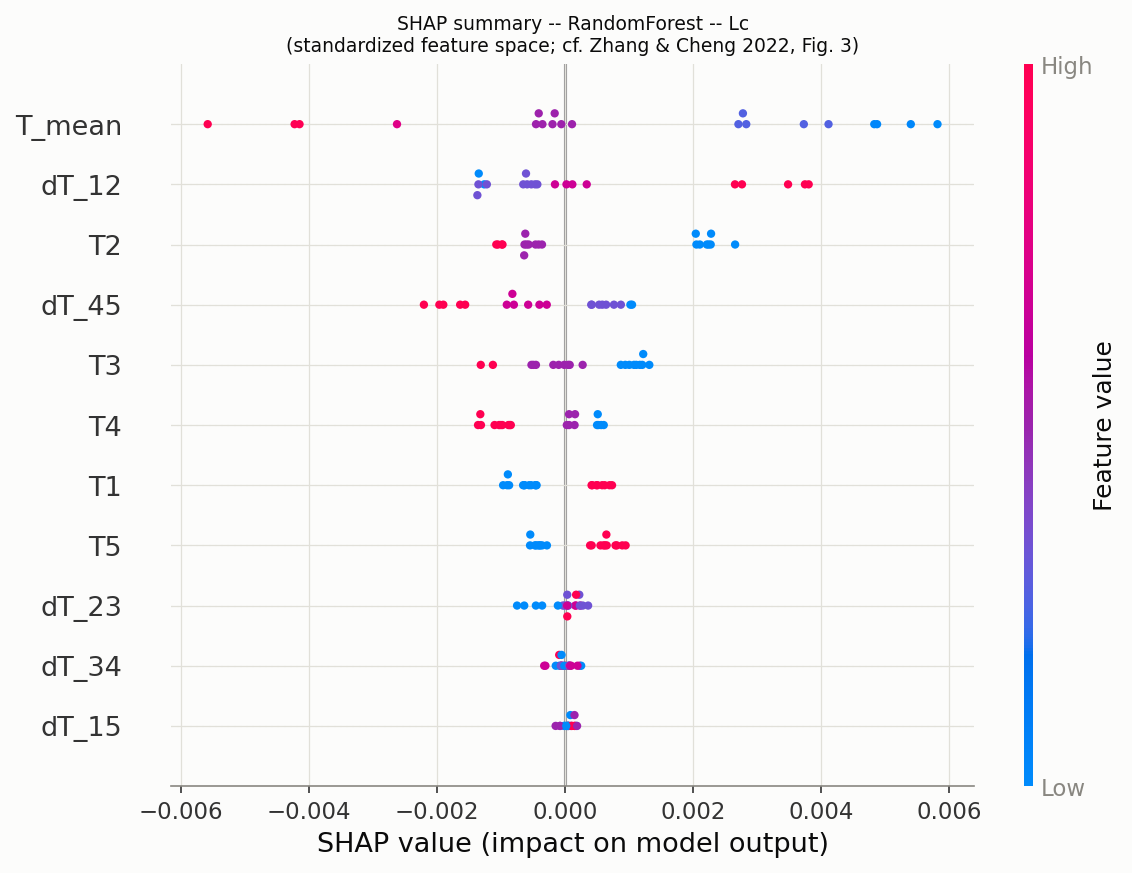
\includegraphics[width=0.48\linewidth]{plots/shap_summary_Lc.png}
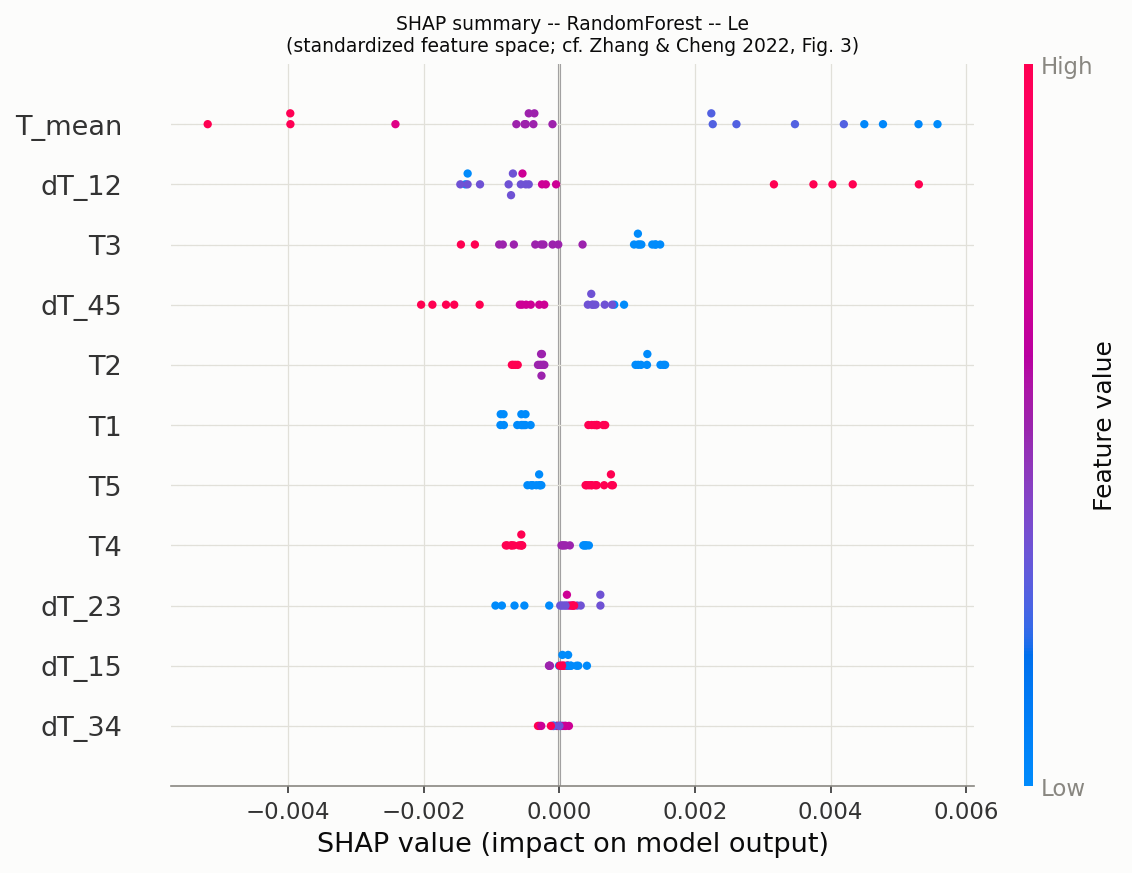
\includegraphics[width=0.48\linewidth]{plots/shap_summary_Le.png}\\[2pt]
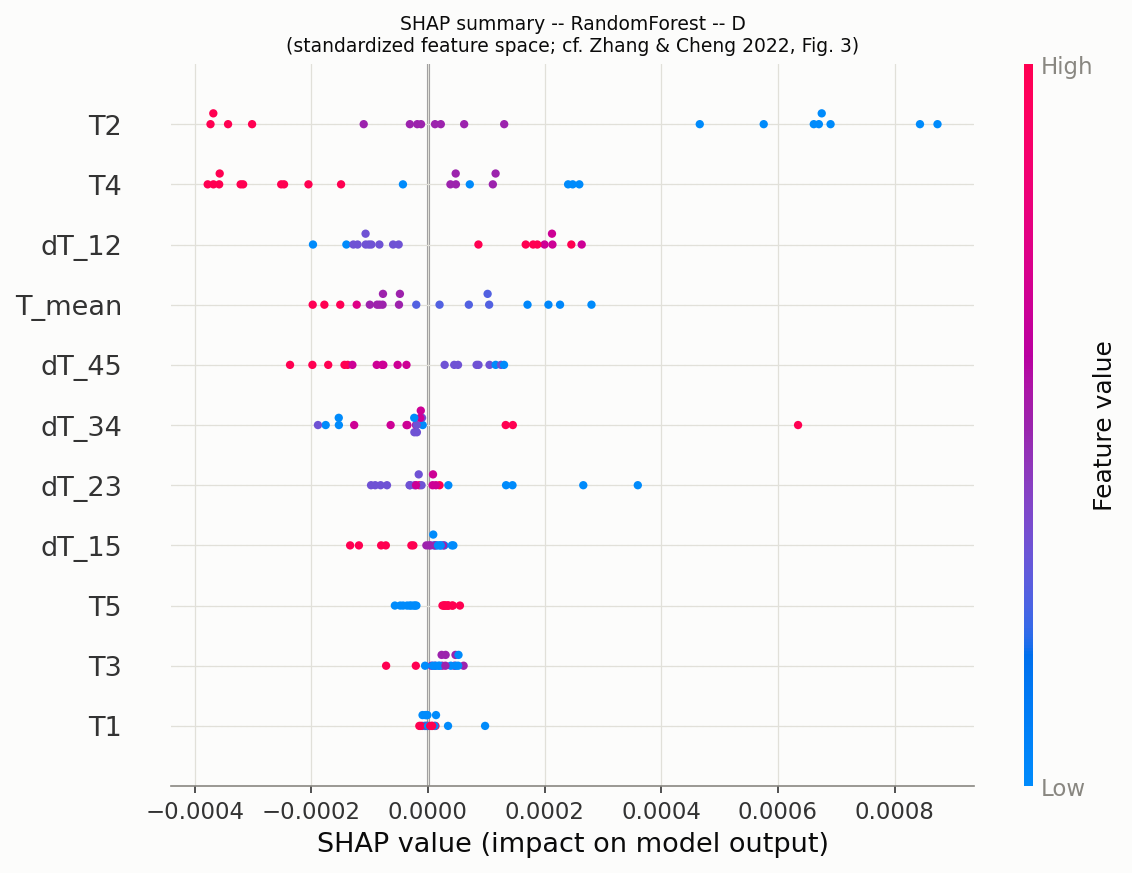
\includegraphics[width=0.48\linewidth]{plots/shap_summary_D.png}
\caption{SHAP summary plots for the random forest model, targets $L_c$, $L_e$ (top), and $D$ (bottom). Color encodes standardized feature value; horizontal position encodes each feature's contribution to that prediction.}
\label{fig:shap}
\end{figure}

\subsection{Automated Inverse Design}
As a demonstration of the optimizer described in Section~IV-H, we specified a target outcome of $D=0$ -- a perfectly flat, undeflected interface, representing minimal radial thermal stress -- and allowed differential evolution to search the training-range-bounded set-point space. Table~\ref{tab:optimization} reports the recommended set-points and the surrogate's predicted outcome.

\begin{table}[!t]
\caption{Automated Inverse Design: Recommended Set-Points for Target $D=0$}
\label{tab:optimization}
\centering
\begin{tabular}{@{}cc c cc@{}}
\toprule
\textbf{Heater} & \textbf{Set-point (K)} & & \textbf{Predicted} & \textbf{Value} \\
\midrule
$T_1$ & 1255.0 & & $L_c$ & $-0.2142$ m \\
$T_2$ & 1235.1 & & $L_e$ & $-0.2145$ m \\
$T_3$ & 1215.1 & & $D$ & $1.8\times10^{-4}$ m \\
$T_4$ & 1075.1 & & $\sigma_D$ & $4\times10^{-6}$ m \\
$T_5$ & 1035.0 & & & \\
\bottomrule
\end{tabular}
\end{table}

The optimizer converges to a predicted deflection of $D\approx0.18\,$mm against a target of exactly zero, with a correspondingly tiny objective value ($3.6\times10^{-8}$) and low predictive uncertainty ($\sigma_D=4\,\mu$m) at the recommended set-point -- indicating the surrogate is confident in this region of the design space, consistent with it lying within the training data's observed range by construction. We emphasize, as the surrogate's own validation logic enforces, that this is a screening-level recommendation from a data-driven approximation of CrysMAS, not a validated furnace control instruction; re-running CrysMAS itself, or a physical trial, at the recommended set-point would be required before acting on it in practice. Nonetheless, this constitutes a fully automated, uncertainty-aware alternative to the reference study's manual, twelve-scenario heuristic check, and can be re-run for arbitrary target outcomes at negligible computational cost.

\subsection{Independent versus Multi-Output Modeling}
Table~\ref{tab:multioutput} compares jointly trained multi-output models against the average of their independently trained per-target counterparts, under identical cross-validation folds. The two approaches perform comparably; independent models were retained for final deployment because per-target model selection allowed a different algorithm to be chosen for each target where warranted (Section~IV-F), which is only knowable by comparing independently in the first place.

\begin{table}[!t]
\caption{Multi-Output versus Independent Modeling (Mean CV $R^2$ Across Targets)}
\label{tab:multioutput}
\centering
\begin{tabular}{@{}lcc@{}}
\toprule
\textbf{Model} & \textbf{Joint (multi-output)} & \textbf{Avg.\ of independent} \\
\midrule
Random Forest & 0.764 & 0.716 \\
XGBoost-family & 0.758 & 0.758 \\
\bottomrule
\end{tabular}
\end{table}

% =================================================================
\section{Limitations}
% =================================================================
This study's conclusions should be interpreted with several limitations in mind. The underlying data is generated entirely by CrysMAS simulation, not physical measurement; every reported number describes model fit to that simulation's output at 96 sampled operating points, not validated agreement with a real furnace. The sample size ($n=96$, with an approximately 77-row training split) is small for a seven-model comparison, and cross-validation statistics -- particularly for the deflection target $D$ -- carry substantial fold-to-fold variance (standard deviations up to 0.27 in $R^2$), meaning single-seed results should be interpreted as indicative rather than precise. The single-target hyperparameter tuning simplification (Section~IV-C) was adopted for stability at this sample size but is not equivalent to a fully nested search. The pooled-versus-reference-study $R^2$ discrepancy for $D$ (Section~V-C) is only partially resolved and its exact remaining cause is not identified. No governing heat-transfer equations are encoded in the surrogate itself, which remains purely data-driven rather than physics-informed. Finally, the automated inverse-design recommendation (Section~V-G) has not been validated against a CrysMAS re-simulation or physical trial, and should be treated as a screening suggestion rather than an operational instruction.

% =================================================================
\section{Conclusion and Future Work}
% =================================================================
This paper presented an uncertainty-aware, explainable machine learning framework for surrogate modeling and automated inverse design of melt-crystal interface control in a five-heater vertical Bridgman furnace, directly extending the only prior machine-learning study on this exact simulation dataset. By independently modeling three physically distinct interface quantities across seven algorithms under rigorous, leakage-free cross-validation, we identified Gaussian process regression as a strictly dominant surrogate that additionally supplies calibrated predictive uncertainty absent from all prior work on this system. By introducing a pooled cross-validation statistic matched to the reference study's own apparent evaluation methodology, we resolved a substantial fraction of an initially observed performance discrepancy while honestly reporting what remained unresolved. By validating our SHAP explanations against the reference study's independently derived SHAP findings, we confirmed cross-study agreement on the physical drivers of interface deflection while demonstrating that engineered thermal-gradient features carry signal the reference study's raw-feature representation could not access. Finally, by replacing a manual, non-systematic heater-adjustment procedure with an automated, uncertainty-penalized optimizer, we demonstrated a practical, reusable path from surrogate model to actionable process recommendation.

Future work should prioritize closing the limitations identified in Section~VI: expanding the underlying simulation design of experiments to reduce cross-validation variance; validating optimizer-recommended set-points against CrysMAS re-simulation or physical trials; and incorporating governing heat-transfer relationships as a physics-informed prior -- for instance, as a structured mean function within the Gaussian process -- to move from a purely data-driven surrogate toward a hybrid digital twin.

\section*{Code and Data Availability}
All source code, trained models, and result tables supporting this paper are openly available in the accompanying repository. The underlying simulation dataset is available at Mendeley Data, DOI: 10.17632/4hr6cx2p8m.1 \cite{zhang_mendeley}.

% =================================================================
% References
% =================================================================
\begin{thebibliography}{00}

\bibitem{bridgman} P. W. Bridgman, ``Nobel Lecture: General Survey of Certain Results in the Field of High-Pressure Physics,'' Nobelprize.org.

\bibitem{zhang_cheng2022} C. Zhang and Q. Cheng, ``Predicting Melt-Crystal Interface Position and Shape during the Manufacturing Process of Single Crystal via Explainable Machine Learning Models,'' \emph{IOP Conf. Ser.: Mater. Sci. Eng.}, vol. 1258, p. 012029, 2022.

\bibitem{zhang_mendeley} C. Zhang, ``Numerical simulation data of melt-crystal interface position and deflection of BaBrCl in a 5-heater vertical Bridgman furnace,'' \emph{Mendeley Data}, V1, 2022. doi: 10.17632/4hr6cx2p8m.1

\bibitem{derby_neutron} J. J. Derby, C. Zhang, J. Seebeck, J. H. Peterson, A. S. Tremsin, D. Perrodin, G. A. Bizarri, E. D. Bourret, and S. C. Vogel, ``Computational modeling and neutron imaging to understand interface shape and solute segregation during the vertical gradient freeze growth of BaBrCl:Eu,'' \emph{J. Cryst. Growth}, vol. 536, p. 125572, 2020.

\bibitem{yan2016} Z. Yan, T. Shalapska, and E. D. Bourret, ``Czochralski growth of the mixed halides BaBrCl and BaBrCl:Eu,'' \emph{J. Cryst. Growth}, vol. 435, pp. 42--45, 2016.

\bibitem{crysmas_manual} \emph{CrysMAS User Manual and Tutorial}, 2013. [Online]. Available: http://www.cglerlangen.com/downloads/Manual.pdf

\bibitem{naumann1982} R. J. Naumann, ``An analytical approach to thermal modeling of Bridgman-type crystal growth: I. One-dimensional analysis,'' \emph{J. Cryst. Growth}, vol. 58, no. 3, pp. 554--568, 1982.

\bibitem{dropka_review} N. Dropka and M. Holena, ``Application of Artificial Neural Networks in Crystal Growth of Electronic and Opto-Electronic Materials,'' \emph{Crystals}, vol. 10, no. 8, p. 663, 2020.

\bibitem{dang2019} Y. Dang, L. Liu, and Z. Li, ``Optimization of the controlling recipe in quasi-single crystalline silicon growth using artificial neural network and genetic algorithm,'' \emph{J. Cryst. Growth}, vol. 522, pp. 195--203, 2019.

\bibitem{takehara2021} Y. Takehara, A. Sekimoto, Y. Okano, T. Ujihara, and S. Dost, ``Explainable machine learning for the analysis of transport phenomena in top-seeded solution growth of SiC single crystal,'' \emph{J. Therm. Sci. Technol.}, vol. 16, no. 1, JTST0009, 2021.

\bibitem{dropka2019} N. Dropka, M. Holena, S. Ecklebe, C. Frank-Rotsch, and J. Winkler, ``Fast forecasting of VGF crystal growth process by dynamic neural networks,'' \emph{J. Cryst. Growth}, vol. 521, pp. 9--14, 2019.

\bibitem{tsunooka2018} Y. Tsunooka, N. Kokubo, G. Hatasa, S. Harada, M. Tagawa, and T. Ujihara, ``High-speed prediction of computational fluid dynamics simulation in crystal growth,'' \emph{CrystEngComm}, vol. 20, pp. 6546--6550, 2018.

\bibitem{lundberg2017} S. M. Lundberg and S.-I. Lee, ``A Unified Approach to Interpreting Model Predictions,'' in \emph{Advances in Neural Information Processing Systems 30}, 2017.

\bibitem{lundberg2020} S. M. Lundberg, G. Erion, H. Chen, et al., ``From local explanations to global understanding with explainable AI for trees,'' \emph{Nat. Mach. Intell.}, vol. 2, pp. 56--67, 2020.

\bibitem{storn1997} R. Storn and K. Price, ``Differential Evolution -- A Simple and Efficient Heuristic for Global Optimization over Continuous Spaces,'' \emph{J. Global Optim.}, vol. 11, pp. 341--359, 1997.

\bibitem{breiman2001} L. Breiman, ``Random Forests,'' \emph{Mach. Learn.}, vol. 45, pp. 5--32, 2001.

\bibitem{chen2016} T. Chen and C. Guestrin, ``XGBoost: A Scalable Tree Boosting System,'' in \emph{Proc. 22nd ACM SIGKDD Int. Conf. Knowledge Discovery and Data Mining}, 2016, pp. 785--794.

\bibitem{rasmussen2006} C. E. Rasmussen and C. K. I. Williams, \emph{Gaussian Processes for Machine Learning}. Cambridge, MA: MIT Press, 2006.

\bibitem{pedregosa2011} F. Pedregosa, G. Varoquaux, A. Gramfort, et al., ``Scikit-learn: Machine Learning in Python,'' \emph{J. Mach. Learn. Res.}, vol. 12, pp. 2825--2830, 2011.

\end{thebibliography}

\end{document}
